%!TEX TS-program = pdflatexmk
%!TEX root = ../handbook.tex

% Copyright 2018 Martin Scheidt (ISC license)
% Permission to use, copy, modify, and/or distribute this file for any purpose with or without fee is hereby granted, provided that the above copyright notice and this permission notice appear in all copies.

\part{\IfLanguage{english}{Manual}\IfLanguage{ngerman}{Anleitung}}

\chapter{\IfLanguage{english}{Setup of a Line}\IfLanguage{ngerman}{Aufbau der Strecke}}
  \noindent
  \IfLanguage{english}{The line consists of any number of spaces. Signals or platforms can be arranged along the line.}
  \IfLanguage{ngerman}{Die Strecke besteht aus einer beliebigen Anzahl von Feldern. An die Strecke können Signale oder Bahnsteigkanten angeordnet werden.}
  \\[0.5cm]
  \tikzfigure{composition.tikz}

\chapter{\IfLanguage{english}{Signal Aspects}\IfLanguage{ngerman}{Signalbegriffe}}
  \noindent
  \IfLanguage{english}{The main signal may only show the proceed aspect if there is no train in the following block section (from track vacancy detector to track vacancy detector).
  The distant signal is located in front of the main signal in braking distance and reflects the signal aspect of the main signal.}
  \IfLanguage{ngerman}{Das Hauptsignal darf nur Fahrt zeigen, wenn im nachfolgenden Blockabschnitt (von Gleisfreimeldegrenze zu Gleisfreimeldegrenze) kein Zug ist.
  Das Vorsignal steht im Bremswegabstand vor dem Hauptsignal und spiegelt den Signalbegriff vom Hauptsignal.}
  \begin{center}
    %!TEX TS-program = pdflatexmk
%!TEX root = ../handbook.tex

% Copyright 2018 RailToolKit (Attribution 4.0 International, CC-BY 4.0)
% You are free to copy and redistribute the material in any medium or format. You are free to remix, transform, and build upon the material for any purpose, even commercially. You must give appropriate credit, provide a link to the license, and indicate if changes were made. You may not apply legal terms or technological measures that legally restrict others from doing anything the license permits. No warranties are given.

\begin{tabular}{rcc}
  \toprule
  & 
    \IfLanguage{english}{halt}
    \IfLanguage{ngerman}{Halt}
  &
    \IfLanguage{english}{proceed}
    \IfLanguage{ngerman}{Fahrt}
  \\
  \hline
    \IfLanguage{english}{main signal}
    \IfLanguage{ngerman}{Hauptsignal}
  &
  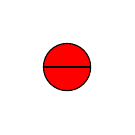
\begin{tikzpicture}[anchor=base,baseline=-3]
    \draw [fill=red] (0,0) circle (0.3);
    \draw (-0.3,0) -- (0.3,0);
    \path (-0.5,-0.5) rectangle ++(1,1); % background rectangle to unify every cell containing a symbol
  \end{tikzpicture} &
  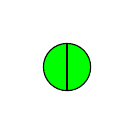
\begin{tikzpicture}[anchor=base,baseline=-3]
    \draw [fill=green] (0,0) circle (0.3);
    \draw (0,-0.3) -- (0,0.3);
    \path (-0.5,-0.5) rectangle ++(1,1); % background rectangle to unify every cell containing a symbol
  \end{tikzpicture}
  \\
    \IfLanguage{english}{distant signal}
    \IfLanguage{ngerman}{Vorsignal}
  &
  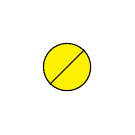
\begin{tikzpicture}[anchor=base,baseline=-3]
    \draw [fill=yellow] (0,0) circle (0.3);
    \draw (-0.22,-0.22) -- ++(0.44,0.44);
    \path (-0.5,-0.5) rectangle ++(1,1); % background rectangle to unify every cell containing a symbol
  \end{tikzpicture} &
  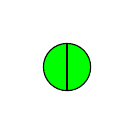
\begin{tikzpicture}[anchor=base,baseline=-3]
    \draw [fill=green] (0,0) circle (0.3);
    \draw (0,-0.3) -- (0,0.3);
    \path (-0.5,-0.5) rectangle ++(1,1); % background rectangle to unify every cell containing a symbol
  \end{tikzpicture} \\
  \bottomrule
\end{tabular}

  \end{center}

\chapter{\IfLanguage{english}{Simulation of Driving Dynamics}\IfLanguage{ngerman}{Simulation der Fahrdynamik}}\label{sec:Simulation_Driving_Dynamics}
  \noindent
  \IfLanguage{english}{The simulation is based on rounds.\\ Each round consists of at least two consecutive steps:}
  \IfLanguage{ngerman}{Die Simulation erfolgt Rundenbasiert.\\ Jede Runde besteht aus mindestens zwei aufeinanderfolgenden Schritten:}
  \begin{enumerate}
    \IfLanguage{english}{
      \item The train makes the movement set in the previous round.
      \item All signals are set according to the track occupancy.
      \item (optional) A new shift lever position can be chosen.
    }
    \IfLanguage{ngerman}{
      \item Der Zug macht die Bewegung, die in der vorhergehenden Runde gesetzt wurde.
      \item Alle Signale werden entsprechend der Gleisbelegung eingestellt.
      \item (optional) Eine neue Schalthebelposition kann gewählt werden.
    }
  \end{enumerate}
  \IfLanguage{english}{At the start of the game, the train stands still. Shift lever positions start at the ``$0$'' field.
  The different train dynamics are depicted by different possible movements of the shift lever.}
  \IfLanguage{ngerman}{Beim Start des Spiels steht der Zug. Schalthebelposition beginnen bei dem Feld ``$0$''.
  Die unterschiedliche Fahrdynamik von Zügen wird durch unterschiedliche mögliche Schalthebelbewegung abgebildet.}

\chapter{\IfLanguage{english}{Example}\IfLanguage{ngerman}{Beispiel}}
  \IfLanguage{english}{The shift lever is moved along the green arrows. Shift lever positions for a passenger train:}
  \IfLanguage{ngerman}{Der Schalthebel wird entlang der grünen Pfeile bewegt. Schalthebelpositionen für einen Personenzug:}
  \begin{center}
    \tikzfigure[0.8\textwidth]{control_lever.tikz}
  \end{center}
  \vspace*{0.5cm}
  \IfLanguage{english}{A train is supposed to accelerate on the following track:}
  \IfLanguage{ngerman}{Ein Zug soll auf folgender Strecke beschleunigen:}
  \\
  \tikzfigure{initial_setup.tikz}
  \\[0.5cm]
  \IfLanguage{english}{ For the course of the learning game, we start with the first round and follow the process from the previous section \emph{\nameref{sec:Simulation_Driving_Dynamics}}.
  In the first round, the train from the initial condition stands still. In the example there are no signals that can be set.
  We can move the shift lever by one position to \SI{40}{\kilo\metre\per\hour} forward. The round is over.}
  \IfLanguage{ngerman}{Für den Verlauf des Lernspiels beginnen wir mit der ersten Runde und befolgen den Ablauf aus vorheringen Abschnitt \emph{\nameref{sec:Simulation_Driving_Dynamics}}.
  In der ersten Runde steht der Zug aus der Anfangsbedingung. Im Beispiel gibt es keine Signale die eingestellt werden können.
  Wir können den Schalthebel um eine Position auf \SI{40}{\kilo\metre\per\hour} nach vorne bewegen. Die Runde ist beendet.}

  \IfLanguage{english}{ The second round begins with the execution of the movement one field to the right.
  The shift lever can be moved on and the round is over.
  The third round begins with the execution of the movement by \emph{two} fields to the right.
  The shift lever can be moved on again and the round is over.
  Continue until the position of \SI{120}{\kilo\metre\per\hour} is reached and the train moves evenly with three fields per round.}
  \IfLanguage{ngerman}{Die zweite Runde beginnt mit dem Ausführen der Bewegung um ein Feld nach rechts.
  Der Schalthebel kann wieder weiterbewegt werden und die Runde ist damit beendet.
  Die dritte Runde beginnt mit dem Ausführen der Bewegung um \emph{zwei} Felder nach rechts.
  Der Schalthebel kann wieder weiterbewegt werden und die Runde ist damit beendet.
  Und so weiter, bis man auf der Position auf \SI{120}{\kilo\metre\per\hour} angekommen ist und der Zug sich gleichmäßig mit drei Felder pro Runde weiter bewegt.}
  \\[0.5cm]
  %!TEX TS-program = pdflatexmk
%!TEX root = ../handbook.tex

% Copyright 2018 Martin Scheidt (ISC license)
% Permission to use, copy, modify, and/or distribute this file for any purpose with or without fee is hereby granted, provided that the above copyright notice and this permission notice appear in all copies.

\begin{tabularx}{0.95\textwidth}{rcccX}
  \toprule
  \IfLanguage{english}{
    Round & current    & 1.Step    & 2.Step      & \\
          & speed      & Move      & shift lever & \\
          &            &           & on          & \\
  }
  \IfLanguage{ngerman}{
    Runde & aktuelle   & 1.Schritt & 2.Schritt   & \\
          & Geschwin-  & Bewegen   & Schalthebel & \\
          & digkeit    & um        & auf         & \\
  }
  \hline
  $1$   &   \SI{0}{\kilo\metre\per\hour} &
  $0$
    \IfLanguage{english}{fields}
    \IfLanguage{ngerman}{Felder}
  &  \SI{40}{\kilo\metre\per\hour} & \tikzfigure[\linewidth]{movement_example1.tikz}
  \\
  $2$   &  \SI{40}{\kilo\metre\per\hour} &
  $1$
    \IfLanguage{english}{field}
    \IfLanguage{ngerman}{Feld}
  &  \SI{80}{\kilo\metre\per\hour} & \tikzfigure[\linewidth]{movement_example2.tikz}
  \\
  $3$   &  \SI{80}{\kilo\metre\per\hour} &
  $2$
    \IfLanguage{english}{fields}
    \IfLanguage{ngerman}{Felder}
  & \SI{120}{\kilo\metre\per\hour} & \tikzfigure[\linewidth]{movement_example3.tikz}
  \\
  $4$   & \SI{120}{\kilo\metre\per\hour} &
  $3$
    \IfLanguage{english}{fields}
    \IfLanguage{ngerman}{Felder}
  & \SI{120}{\kilo\metre\per\hour} & \tikzfigure[\linewidth]{movement_example4.tikz}
  \\
  $5$   & \SI{120}{\kilo\metre\per\hour} &
  $3$
    \IfLanguage{english}{fields}
    \IfLanguage{ngerman}{Felder}
  & \SI{120}{\kilo\metre\per\hour} & \tikzfigure[\linewidth]{movement_example5.tikz}
  \\
  etc. & & & & \\
  \bottomrule
\end{tabularx}


  
